\documentclass[12pt, oneside]{article}
\usepackage[letterpaper, margin=1in, headsep=0.5in, left=0.3in, right=2.5in]{geometry}
\usepackage[english]{babel}
\usepackage[utf8]{inputenc}
\usepackage{amsmath}
\usepackage{amsfonts}
\usepackage{amssymb}
\usepackage{tikz}
\usepackage{yhmath}
\usetikzlibrary{quotes, angles}
\usepackage{graphicx}
\usepackage{enumitem}
\usepackage{multicol}

\newif\ifmeta
\metatrue %print standards and topics tags

\title{Regents Geometry}
\author{Chris Huson}
\date{April 2022}

\usepackage{fancyhdr}
\pagestyle{fancy}
\fancyhf{}
\renewcommand{\headrulewidth}{0pt} % disable the underline of the header
\raggedbottom

%\fancyhead[LE]{\thepage}
\fancyhead[RO]{Name:}
\fancyhead[LO]{BECA / Dr. Huson / Geometry Regents Mixed Review}
\cfoot{\thepage}

\begin{document}
\subsubsection*{11.11 Similar triangles \hfill HSG.SRT.B.5}
\begin{enumerate}[itemsep=1.7cm]
%\subsubsection*{Similarity \hfill January 2020}
\item Triangle $ABC$ is similar to triangle $DEF$. Which statement is \emph{not}
always true?
\begin{multicols}{2}
  \begin{enumerate}
    \item $\angle B \cong \angle E$
    \item $\angle C \cong \angle D$ 
    \item $\angle A \cong \angle D$
    \item $\angle C \cong \angle F$
  \end{enumerate}
\end{multicols}


\item From a boat on the water three-quarters of a mile from the base of a lighthouse, the angle of elevation to its top is $2.74^\circ$. To the nearest foot, what is the height of the lighthouse? (1 mile = 5280 feet)
\vspace{1cm}

\item In trapezoid $ABCD$ below, $\overline{AB} \parallel \overline{CD}$.
\begin{center}
  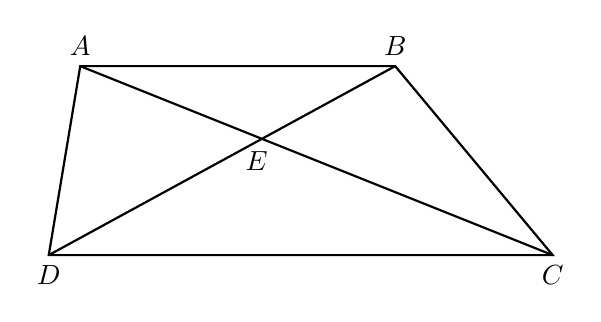
\begin{tikzpicture}[scale=0.8]
    \draw [-, thick] 
      (0,0)node[below]{$D$}--
      (8,0)node[below]{$C$}--
      (5.5,3)node[above]{$B$}--
      (0.5,3)node[above]{$A$}--cycle;
    \draw [-, thick] (0,0)--(5.5,3);
    \draw [-, thick] (0.5,3)--(8,0);
    \node at (3.3, 1.5){$E$};
  \end{tikzpicture}
  \end{center}
If $AB=11.7$, $BE=5.4$, and $CD=15.6$, what is the length of $\overline{BD}$?
\vspace{1cm}

\item The area of a sector of a circle with diameter measuring 10 cm is $3.75\pi \; \rm{cm}^2$. What is the measure of the central angle that forms the sector?

\newpage
\item The equation of a cirle is $x^2+y^2-2x-14y=-14$. What are the center and radius of the circle? \vspace{1cm}

\item In the accompanying diagram of right triangle $ABC$, altitude $\overline{BD}$ is drawn to hypotenuse $\overline{AC}$.
  \begin{center}
    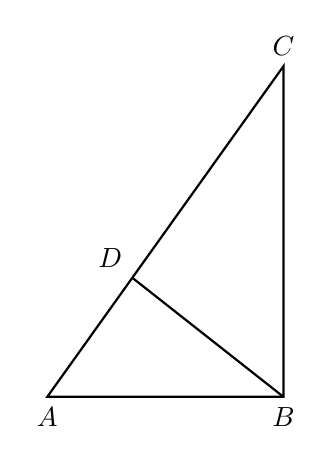
\begin{tikzpicture}[scale=0.6]
    \draw [thick]
    (0,0)node[below]{$A$}--
    (5,0)node[below]{$B$}--
    (5,7)node[above]{$C$}--cycle;
    \draw [thick](1.8,2.52)node[above left]{$D$}--(5,0);
  \end{tikzpicture}
  \end{center}
  Which statement must be true?
  \begin{multicols}{2}
    \begin{enumerate}
      \item $\displaystyle \frac{AB}{BC} = \frac{BD}{AC}$
      \item $\displaystyle \frac{BC}{AC} = \frac{AD}{AB}$
      \item $\displaystyle \frac{AD}{AB} = \frac{AB}{AC}$ 
      \item $\displaystyle \frac{BD}{BC} = \frac{AB}{AD}$
    \end{enumerate}
  \end{multicols}

\item In the diagram of $\triangle ABC$ below, points $D$ and $E$ are on sides $\overline{AB}$ and $\overline{CB}$ respectively, such that $\overline{DE} \parallel \overline{AC}$.
\begin{center}
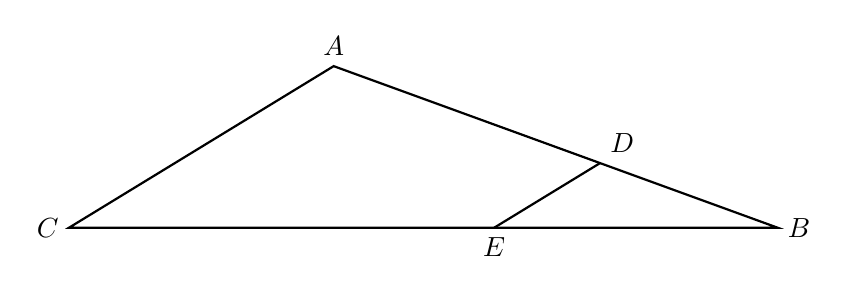
\begin{tikzpicture}[scale=0.6]
  \draw [thick]
  (0,0) node[right] {$B$}--
  (160:10) node[above] {$A$}--
  (-15,0) node[left] {$C$}--cycle;
  \draw [thick]
  (160:4) node[above right] {$D$}--
  (-6,0) node[below] {$E$};
\end{tikzpicture}
\end{center}
IF $DB$ is 2 less than $EB$, $AB=18$, and $BC=24$, what is the length of $\overline{CE}$?

\end{enumerate}
\end{document}
  